\documentclass[10pt]{beamer}

% Beamer style
%\usetheme[secheader]{Madrid}
% \usetheme{CambridgeUS}
\useoutertheme{infolines}
\usecolortheme[rgb={0.65,0.15,0.25}]{structure}
% \usefonttheme[onlymath]{serif}
\beamertemplatenavigationsymbolsempty
%\AtBeginSubsection

% Packages
%\usepackage[french]{babel}
\usepackage[latin1]{inputenc}
\usepackage{color}
\usepackage{xspace}
\usepackage{dsfont, stmaryrd}
\usepackage{amsmath, amsfonts, amssymb}
\usepackage{epsfig}
\usepackage{url}
\usepackage{/home/robin/LATEX/Biblio/astats}
%\usepackage[all]{xy}
\usepackage{graphicx}

% Commands
\definecolor{darkred}{rgb}{0.65,0.15,0.25}
\newcommand{\emphase}[1]{\textcolor{darkred}{#1}}
% \newcommand{\emphase}[1]{{#1}}
\newcommand{\paragraph}[1]{\textcolor{darkred}{#1}}
\newcommand{\refer}[1]{{{\textcolor{blue}{{[\cite{#1}]}}}}}
\newcommand{\Refer}[1]{{{\textcolor{blue}{{[#1]}}}}}
\renewcommand{\newblock}{}

% Symbols
\newcommand{\Abf}{{\bf A}}
\newcommand{\Beta}{\text{B}}
\newcommand{\Bcal}{\mathcal{B}}
\newcommand{\BIC}{\text{BIC}}
\newcommand{\Ccal}{\mathcal{C}}
\newcommand{\dd}{\text{~d}}
\newcommand{\dbf}{{\bf d}}
\newcommand{\Dcal}{\mathcal{D}}
\newcommand{\Esp}{\mathbb{E}}
\newcommand{\Ebf}{{\bf E}}
\newcommand{\Ecal}{\mathcal{E}}
\newcommand{\Gcal}{\mathcal{G}}
\newcommand{\Gam}{\mathcal{G}\text{am}}
\newcommand{\Hcal}{\mathcal{H}}
\newcommand{\Ibb}{\mathbb{I}}
\newcommand{\Ibf}{{\bf I}}
\newcommand{\ICL}{\text{ICL}}
\newcommand{\Cov}{\mathbb{C}\text{ov}}
\newcommand{\Corr}{\mathbb{C}\text{orr}}
\newcommand{\Var}{\mathbb{V}}
\newcommand{\Vsf}{\mathsf{V}}
\newcommand{\pen}{\text{pen}}
\newcommand{\Fcal}{\mathcal{F}}
\newcommand{\Hbf}{{\bf H}}
\newcommand{\Jcal}{\mathcal{J}}
\newcommand{\Kbf}{{\bf K}}
\newcommand{\Lcal}{\mathcal{L}}
\newcommand{\Mcal}{\mathcal{M}}
\newcommand{\mbf}{{\bf m}}
\newcommand{\mum}{\mu(\mbf)}
\newcommand{\Ncal}{\mathcal{N}}
\newcommand{\Nbf}{{\bf N}}
\newcommand{\Nm}{N(\mbf)}
\newcommand{\Ocal}{\mathcal{O}}
\newcommand{\Obf}{{\bf 0}}
\newcommand{\Omegas}{\underset{s}{\Omega}}
\newcommand{\Pbf}{{\bf P}}
\newcommand{\Pt}{\widetilde{P}}
\newcommand{\Pcal}{\mathcal{P}}
\newcommand{\Qcal}{\mathcal{Q}}
\newcommand{\Rbb}{\mathbb{R}}
\newcommand{\Rcal}{\mathcal{R}}
\newcommand{\Scal}{\mathcal{S}}
\newcommand{\Tcal}{\mathcal{T}}
\newcommand{\Ucal}{\mathcal{U}}
\newcommand{\Vcal}{\mathcal{V}}
\newcommand{\BP}{\text{BP}}
\newcommand{\EM}{\text{EM}}
\newcommand{\VEM}{\text{VEM}}
\newcommand{\VBEM}{\text{VBEM}}
\newcommand{\cst}{\text{cst}}
\newcommand{\obs}{\text{obs}}
\newcommand{\ra}{\emphase{\mathversion{bold}{$\rightarrow$}~}}
%\newcommand{\transp}{\text{{\tiny $\top$}}}
\newcommand{\transp}{\text{{\tiny \mathversion{bold}{$\top$}}}}
\newcommand{\logit}{\text{logit}\xspace}

% Directory
\newcommand{\fignet}{/home/robin/Bureau/RECHERCHE/RESEAUX/EXPOSES/FIGURES}
\newcommand{\figchp}{/home/robin/Bureau/RECHERCHE/RUPTURES/EXPOSES/FIGURES}


%====================================================================
%====================================================================

%====================================================================
%====================================================================
\begin{document}
%====================================================================
%====================================================================

%====================================================================
\title[Exact inference with discrete parameters]{Exact Bayesian inference for some models with discrete parameters}

\author[S. Robin]{S. Robin \\ ~\\
  \begin{tabular}{ll}
    Joint work with & A. Cleynen, E. Lebarbier, G. Rigaill, \\
    & L. Schwaller, M. Stumpf
  \end{tabular}
  }

\institute[INRA/AgroParisTech]{INRA / AgroParisTech \\
  \vspace{-.1\textwidth}
  \begin{tabular}{ccccc}
    
\includegraphics[height=.3\textheight]{\fignet/LogoINRA-Couleur} & 
    \hspace{.02\textheight} &
    
\includegraphics[height=.08\textheight]{\fignet/logagroptechsolo} & 
    \hspace{.02\textheight} &
    
\includegraphics[height=.09\textheight]{\fignet/logo-ssb}
    \\ 
  \end{tabular} \\
  \bigskip
  }

\date[EDMH '16]{EDMH, September 2016, IHES, Bures-sur-Yvette}

%====================================================================
%====================================================================
\maketitle
%====================================================================

%====================================================================
%====================================================================
\section{Bayesian inference with discrete parameters}
%====================================================================
\frame{\frametitle{General framework 1/2}

  \paragraph{A typical goal of statistical inference.} Infer the laws that have undergone the generation of observed data $Y$.

  \bigskip \bigskip \pause
  \paragraph{A statistical model} encodes these laws in a probability distribution $p$:
  $$
  \text{\emphase{Model:}} \qquad Y \sim p
  $$

  \bigskip \pause
  \paragraph{Statistical inference:} Based on observation $Y_1, \dots, Y_n$, try to infer $p$:
  $$
  \widehat{p} = \Fcal(Y_1, \dots, Y_n)
  $$
  
  \bigskip \pause
  \paragraph{Parametric statistical inference:} Assume that $p$ is parametrized with $\vartheta$: $p(\cdot) = p(\cdot; \vartheta)$
  $$
  \text{\emphase{Estimator:}} \qquad \widehat{\vartheta} = \Gcal(Y_1, \dots, Y_n)  
  $$

}
%====================================================================
\frame{\frametitle{General framework 2/2} 

  \paragraph{Bayesian inference:}
  \begin{align*}
   \text{prior:} & \quad p(\vartheta) \\
   \text{likelihood:} & \quad p(Y|\vartheta) \\
   \text{\ra posterior:} & \quad p(\vartheta|Y)
  \end{align*}
  
  \bigskip \pause
  \paragraph{3 main approaches}
  \begin{enumerate}
   \item \pause {Sampling} (MC, MCMC, SMC, IS, ...): get
   $
   (\vartheta^b) \sim p(\vartheta | Y).
   $ \\~ 
   \item \pause {Approximation} (e.g. VB, EP, ...): find
   $
   q_Y(\vartheta) \simeq p(\vartheta | Y).
   $ \\~ 
   \item \pause {Exact:} actually compute
   $
   p(\vartheta|Y)
   $
   or some marginal of interest.
  \end{enumerate}
  }

%====================================================================
\frame{\frametitle{Models with discrete parameters}

  \paragraph{Mixed parameter:} $ \vartheta = (\theta, T)$
  $$
  \theta \in \Theta = \text{continuous set}, 
  \qquad
  T \in \Tcal = \text{discrete (countable) set}, 
  $$
  $$
  \Rightarrow \qquad p(Y) = \emphase{\sum_{T \in \Tcal}} \int_\Theta p(Y, \theta, T) \dd \theta
  $$

  \bigskip \bigskip \pause
  \paragraph{Size of $\Tcal$.}
  \begin{itemize}
   \item No big deal of $\Tcal$ is small (e.g. model selection within a small collection).
%    $$
%    p(T|Y) = \int_\Theta p(Y, \theta, T) \dd \theta \left/ \sum_{T' \in \Tcal} \int_\Theta p(Y, \theta, T') \dd \theta \right.
%    $$
  \\ ~
   \item Big issue if $|\Tcal|$ grows (super-)exponentially with the number of observations $n$ or the number of variables $p$.
  \end{itemize}

}

%====================================================================
\frame{\frametitle{Main issue}

  The calculation of 
  $$
  \sum_{T \in \Tcal}
  $$
  can often not be achieved in a naive way because of the combinatorial complexity\footnote{The frequentist counterpart often raises similar issues.}. 
  \begin{center}
   \ra Need to find algorithmic or algebraic shortcuts\footnote{Supposing that $\int_\Theta$ raises no specific issues (e.g. conjugate priors).}
  \end{center}
  
  \bigskip \pause
  \paragraph{2 examples.}
  \begin{itemize}
   \item Change-point detection \\~
   \item 'Network inference' = inference of the structure of a graphical model
  \end{itemize}
  }

%====================================================================
%====================================================================
\section{Change-point detection}
\frame{\frametitle{Outline} \tableofcontents[currentsection]}

%====================================================================
\subsection*{Change-point detection model}
%====================================================================
\frame{\frametitle{A change-point detection model} 
  \begin{tabular}{cc}
    \hspace{-.5cm}
    \begin{tabular}{p{.5\textwidth}}
      \onslide+<1->{\paragraph{Model.} 
        \begin{itemize}
        \item \onslide+<2->{$K$ segments \\~}
        \item \onslide+<3->{$T = (\tau_k)_k$ change points\\~\\
        $r_k = \llbracket\tau_{k-1}+1; \tau_k\rrbracket$\\~}
        \item \onslide+<4->{$\theta = (\theta_k)_k$ parameters\\~}
        \item \onslide+<5->{$Y = (Y_t)_{1 \leq t \leq n}$ observed data \\~\\
        $Y^r = (Y_t)_{t \in r}$}
        \end{itemize}}
    \end{tabular}
    & 
    \hspace{-1cm}
    \begin{tabular}{c}
	 \hspace{-6cm}
	 \onslide+<5->{$\{Y^r\}_r \text{ indep}, \quad Y^r \sim p(\cdot | \theta_r)$}
	 \\
      \begin{overprint}
        \onslide<2>
        \includegraphics[width=.5\textwidth]{\figchp/FigSeg-Budapest-1} 
        \onslide<3>
        \includegraphics[width=.5\textwidth]{\figchp/FigSeg-Budapest-2} 
        \onslide<4>
        \includegraphics[width=.5\textwidth]{\figchp/FigSeg-Budapest-3} 
        \onslide<5>
        \includegraphics[width=.5\textwidth]{\figchp/FigSeg-Budapest-4} 
        \onslide<6->
        \includegraphics[width=.5\textwidth]{\figchp/FigSeg-Budapest-0} 
      \end{overprint}
    \end{tabular}
  \end{tabular}

  \onslide+<6->{
  \paragraph{Bayesian version:} on the top of this, add
  $
  p(K), p(T|K), p(\theta|K).
  $
  } 

}

%====================================================================
\subsection*{Maximum likelihood inference}
\frame{\frametitle{Maximum likelihood inference (1/2)} 

  \paragraph{Log-likelihood:}
  $$
  \log p(Y; \theta, T) = \sum_{r \in T} \log p(Y^r; \theta^r)
  $$
  
  \pause
  \paragraph{Inference}
  \begin{itemize}
   \item continuous part ($\theta$):
   $$
   \widehat{\theta}_r = \arg\max_{\theta_r} \; \log p(Y^r; \theta^r)
   \qquad \text{standard MLE}
   $$
   \item \pause discrete part ($T$):
   $$
   \widehat{T} = \arg\max_{T} \; \sum_{r \in T} \log p(Y^r; \widehat{\theta}^r)
   = \arg\max_{T} \; \sum_{r \in T} \log \widehat{p}(Y^r)
   $$
   \ra discrete optimization problem
   \end{itemize}
}

%====================================================================
\frame{\frametitle{Maximum likelihood inference (2/2)} 

  \paragraph{Segmentation space} $\Tcal = \Tcal_{1:n}^K =$ set of all possible segmentations of $\llbracket 1; n \rrbracket$ with $K$ segments:
  $$
  |\Tcal| = \binom{n-1}{K-1} \approx \left(\frac{n}{K}\right)^K
  $$
  \ra exhaustive search is prohibited.

  \bigskip \pause
  \paragraph{Dynamic programming} allows to retrieve $\widehat{T}$ in $O(Kn^2)$ \refer{AuL89} using 
  $$
  \max_{T \in \Tcal_{1:j}^K} \sum_{r \in T} \log \widehat{p}(Y^r)
  =
  \max_{K-1 \leq \emphase{i} < j} \left(\max_{T \in \Tcal_{1:\emphase{i}}^{K-1}} \sum_{r \in T} \log
  \widehat{p}(Y^r)\right) + \log \widehat{p}(Y^{\llbracket \emphase{i}+1; j\rrbracket})
  $$

  \bigskip \bigskip \pause
  Still, further inference is hard to achieve \\
  \ra Standard likelihood theory does not apply to discrete parameters \\
  \qquad (no simple confidence intervals for the $\tau_k$). \\
  \ra Bayesian inference can circumvent some difficulties.
  }
%====================================================================
\subsection*{Bayesian inference}
\frame{\frametitle{Bayesian inference} 

  \paragraph{Factorability assumptions} 
  \begin{itemize}
  \item Prior distribution for the segmentation:
  $$
  p(T|K) = \prod_{r \in T} a(r) , \qquad \text{e.g. } a(r) = n_r^\alpha
  $$
  ~
  \item Independent parameters in each segment ('hyper-Markov' assumption):
  $$
  p(\theta|T) = \prod_{r \in T} p(\theta_r)
  $$
  ~
  \item Data are independent from one segment to another
  $$
  p(Y | T, \theta) = \prod_{r \in T} p(Y^r | \theta_r) 
  $$
  \end{itemize}

}

%====================================================================
\frame{ \frametitle{Some quantities of interest}

  \paragraph{Marginal likelihood.}
  $$
  p(Y|K) 
%   = \sum_{T \in \Tcal^K} \int p(Y, \theta, T | K) \dd \theta 
  \propto \sum_{T \in \Tcal^K} \prod_{r \in T} a(r) p(Y^r)
  $$
  where $p(Y^r) = \int p(Y^r|\theta_r) p(\theta^r) \dd \theta_r$(\footnote{supposed to be easy to compute using e.g. conjugate priors}) and the normalizing constant is
  $$
  \sum_{T \in \Tcal^K} \prod_{r \in T} a(r).
  $$

  \pause \bigskip
  \paragraph{Posterior distribution of a change-point.}
  $$
  \Pr\{\tau_k = t | Y, K\} \propto \left(\sum_{T \in \Tcal^k_{1:t}} \prod_{r \in T} a(r) p(Y^r) \right) \left(\sum_{T \in \Tcal^{K-k}_{t+1:n}} \prod_{r \in T} a(r) p(Y^r) \right)
  $$

}

%====================================================================
\frame{ \frametitle{Summing over segmentations \refer{RLR11}}

  \paragraph{Property:} {\sl 
%   To compute
%   $$
%   \sum_{T \in \Tcal^K_{1:n}} \prod_{r \in T} f(r),
%   $$
  Define the upper triangular $(n+1) \times (n+1)$ matrix $A$:
  $$
  A_{i, j+1} = f(\llbracket i, j \rrbracket ), \qquad 1 \leq i < j \leq n
  $$ \pause
  Then 
  $$
  \left[A^K\right]_{1,n+1} = \sum_{T \in \Tcal^K_{1:n}} \prod_{r \in T} f(r)
  $$
  \ra all terms are computed in {$O(K n^2)$}. }
  
  \bigskip
  \begin{itemize}
   \item \pause To compute $p(Y)$, take $f(r) = a(r) p(Y^r)$. 
   \item Similar ideas in \refer{Fea06}. 
   \item \pause 'sum-product' = counterpart of 'max-sum' in the dynamic programming algorithm.
  \end{itemize}
  
  \bigskip \pause
  \ra R package EBS (exact Bayesian segmentation) \refer{ClR14}

  }

%====================================================================
\frame{\frametitle{Illustration: Of exons, introns and UTR's}
  
  Regions for a same gene are not adjacent along the genome 
  $$
  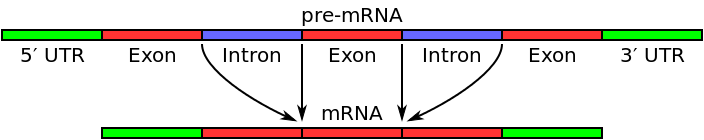
\includegraphics[width=.8\textwidth]{\figchp/Pre-mRNA_to_mRNA}
  $$
  \Refer{Wikipedia}
  
  \bigskip \bigskip \pause
  \begin{itemize}
   \item The transcribed regions are made of both exons and untranslated regions (UTR)
   \item Alternative splicing: some exons can be skipped or the boundaries may vary.
  \end{itemize}

  }

%====================================================================
\frame{\frametitle{Posterior distribution of transcript boundaries in yeast}

  \vspace{-.05\textheight}
  \begin{tabular}{p{.2\textwidth}p{.7\textwidth}}
    \begin{tabular}{p{.3\textwidth}}
	 \paragraph{RNA-seq data:} \\
	 \\ ~\\
	 One gene \\
	 \\
	 $\times$ \\
	 \\
	 Three growth \\
	 conditions \\ 
	 $A$, $B$, $C$
    \end{tabular}
    &
    \begin{tabular}{p{.7\textwidth}}
    \includegraphics[width=.7\textwidth]{\figchp/compyeastresult.pdf}
    \end{tabular}
  \end{tabular}
}

%====================================================================
\frame{\frametitle{Comparing change-point locations \refer{ClR14}}

  \paragraph{One series.} We know how to compute (in $O(Kn^2)$)
  $$
  \Pr\{\tau_k = t | Y, K\} \qquad \text{or} \qquad \Pr\{\tau_k = t | Y\}.
  $$
  
  \bigskip \bigskip \pause
  \paragraph{Two series ($Y�, Y^B$):} Consider the shift of the $k$th change-point 
  $$
  \Pr\{\tau^A_k - \tau^B_k = 0 | Y^A, Y^B, K^A, K^B\}
  $$
  
  \bigskip \bigskip \pause
  \paragraph{$I$ series ($Y^1, \dots Y^I$):} Check if the $k$th change-point is conserved\footnote{Requires a probability change, as $Y^1, \dots Y^I$ are not independent conditionally on $\tau^1_k = \dots = \tau^I_k$.}:
  $$
  \Pr\{\tau^1_k = \dots = \tau^I_k | Y^1, \dots Y^I, K^1, \dots, K^I\}
  $$
  
}

%====================================================================
\frame{\frametitle{Boundary shifts between conditions}

  3 comparisons ($A/B$, $A/C$, $B/C$) $\times$ 4 change points:
  
\centerline{\includegraphics[width=.8\textwidth, height=.8\textheight]{\figchp/cred-yeast.pdf}}

}

%====================================================================
\frame{\frametitle{Comparing transcript boundaries}

Setting $\Pr\{\tau^A_k = \tau^B_k | K\} = 1/2$.

$$
\begin{array}{lccccc}
& \tau_1 & \tau_2 & \tau_3 & \tau_4 \\ 
\hline \\
\Pr\{\tau^A_k = \tau^B_k | Y, K\} & 0.32 & 0.30 &0.99 & 10^{-5} \\ \\
\Pr\{\tau^A_k = \tau^C_k | Y, K\} & 4 \; 10^{-4} & 0.99 &0.99 & 6 \; 10^{-3} \\ \\
\Pr\{\tau^B_k = \tau^C_k | Y, K\} & 5 \; 10^{-2} & 0.60 & 0.99 & 0.99 \\ \\
\Pr\{\tau^A_k = \tau^B_k = \tau^C_k | Y, K\} & 10^{-3} & 0.99  & 0.99 & 6 \; 10^{-3} \\ 
\end{array}
$$

\bigskip
\ra Differences at the UTR's end but not at internal exon boundaries.
}

%====================================================================
\frame{\frametitle{Various isoforms in yeast?} 

  \paragraph{$\Pr\{\tau^A_k = \tau^B_k = \tau^C_k | Y, K\}$} for all yeast genes with 2 expressed exons
  $$
  \begin{tabular}{cc}
  \includegraphics[width=.4\textwidth]{\figchp/statall-all} 
  & 
  \includegraphics[width=.4\textwidth]{\figchp/statall2} 
  \\
   $p_0 = (.5, \;.5, \;.5, \;.5)$
   &
   $p_0 = (.9, \;.99, \;.99, \;.9)$
  \end{tabular}
  $$
}

%====================================================================
%====================================================================
\section{Network inference}
\frame{\frametitle{Outline} \tableofcontents[currentsection]}
%====================================================================
\subsection*{Graphical model framework}
\frame{\frametitle{Graphical model framework} 

  \paragraph{Property [Hammersley-Clifford].} The joint distribution $p(Y) = p(Y_1, \dots Y_p)$ is Markov wrt the (decomposable) graph $G$ iff it factorizes wrt the maximal cliques of $G$:
  $$
  p(Y) \propto \prod_{C \in \Ccal(G)} \psi(Y^c), 
  \qquad Y^c = (Y_j)_{j \in C}.
  $$
  
  \bigskip 
  \ra $G$ reveals the structure of conditional independences between the variables $Y_1, \dots Y_p$.
  
  \bigskip \bigskip \pause
  \paragraph{'Network inference' problem:} Based on $\{(Y_{i1}, \dots Y_{ip})\}_i$ iid $\sim p$, infer $G$.
}

%====================================================================
\frame{\frametitle{Tree-structured network} 

  Suppose the graph $G$ is a tree $T$, $p(Y)$ is Markov wrt $T$ iff
  \begin{eqnarray*}
   p(Y|\theta) 
%    & = & \prod_j p(Y_j|\theta_j) \prod_{(j, k) \in T} \frac{p(Y_j, Y_k|\theta_{jk})}{p(Y_j|\theta_j)p(Y_k|\theta_k)} \\
   & = & \prod_{(j, k) \in T} p(Y_j, Y_k|\theta_{jk}) \left/ \prod_j p^{d_j-1}(Y_j|\theta_j) \right.
  \end{eqnarray*}
  where $d_j$ is the degree (number of neighbors in $T$) of node $j$.
  
  \bigskip \bigskip \pause
  \paragraph{Tree structure assumption.}
  \begin{itemize}
   \item Consistent (although much stronger) with the usual assumption that the graph is sparse. \\~
   \item Not true in general, but may be sufficient for the \emphase{inference on local structures}, such as the existence of a given edge.
  \end{itemize}

}

%====================================================================
\subsection*{Maximum likelihood inference}
\frame{\frametitle{Maximum likelihood inference (1/2)} 

  \paragraph{Log-likelihood.}
  $$
  \log p(Y; \theta, T) = \sum_{(j, k) \in T} \log p(Y_j, Y_k|\theta_{jk}) - \sum_j ({d_j-1}) \log p(Y_j|\theta_j)
  $$
  
  \bigskip \pause
  \paragraph{Inference:}
  \begin{itemize}
   \item continuous part ($\theta$): MLE
   $$
   \widehat{\theta}_j = \arg\max_{\theta_j} \log p(\{Y_{ij}\}_i; \theta_j), 
   \quad
   \widehat{\theta}_{jk} = \arg\max_{\theta_{jk}} \log p(\{(Y_{ij}, Y_{ik})\}_i; \theta_{jk})
   $$
   \item discrete part ($T$)
   $$
   \widehat{T} = \arg\max_T \sum_{(j, k) \in T} \log \frac{p(Y_j, Y_k|\widehat{\theta}_{jk})}{p(Y_j|\widehat{\theta}_j)p(Y_k|\widehat{\theta}_k)}  $$
  \end{itemize}
}

%====================================================================
\frame{\frametitle{Maximum likelihood inference (2/2)} 

  \paragraph{Chow \& Liu algorithm \refer{ChL68}:} Taking
  $$
  f(j, k) = \log p(Y_j, Y_k|\widehat{\theta}_{jk}) - \log p(Y_j|\widehat{\theta}_j) - \log p(Y_k|\widehat{\theta}_k)
  $$
  as the weight of edge $(j, k)$, 
  $$
  \widehat{T} = \arg\max_T \sum_{(j, k) \in T} f(j, k)
  $$
  is the \emphase{maximum spanning tree} with weights $\{f(j, k)\}$, which can be retrieved by Kruskal's algorithm in $O(p^2)$ \refer{Kru56}.
  
  \pause \bigskip \bigskip
  Retrieves the maximum likelihood tree but with no measure of uncertainty. \\
  \ra Exploring the whole tree space allows to evaluate uncertainty. \\
  \ra Bayesian inference can again be a solution.
  }
  
%====================================================================
\subsection*{Bayesian inference}
\frame{\frametitle{Bayesian setting \refer{SRS15}} 

  \bigskip 
  \hspace{-.02\textwidth}\begin{tabular}{lrlcrl}
  \paragraph{Model: \qquad } 
  & prior on $T$: & $\quad p(T) $ \\
  & prior on $\theta$: & $\quad p(\theta|T)$ & \ra & posterior: & $\quad p(T|Y)$ \\
  & likelihood: & $\quad p(Y|\theta, T)$
  \end{tabular}
  
  \bigskip \bigskip \pause
  \paragraph{Prior on $T$:} factorizes over the edges:
  $$
  p(T) \propto \prod_{(j, k) \in T} a(j, k)
  $$
  
  \bigskip \pause
  \paragraph{Prior on $\theta$:} displays factorability properties, i.e. needs to satisfy
  $$
  p(\theta_{jk}|T) \equiv p(\theta_{jk}) \quad \text{for all } T \ni (j, k).
  $$ 
  \ra Compatible family of strong Markov hyper-distributions \refer{DaL93}:	multinomial-Dirichlet (conjugacy), normal-Wishart (conjugacy), Gaussian copulas (numerical integration), ...?

}

%====================================================================
\frame{\frametitle{Quantities of interest}

  \paragraph{Marginal distribution.}
  $$
  p(Y) \propto 
%   \sum_{T \in \Tcal} \prod_{j, k} \frac{a(j, k) \int p(Y_j, Y_k, \theta_{jk}) \dd \theta_{jk}}{\int p(Y_j, \theta_j) \dd \theta_j \times \int p(Y_k, \theta_k) \dd \theta_k}
  \sum_{T \in \Tcal} \prod_{j, k} \frac{a(j, k) p(Y_j, Y_k) }{p(Y_j) p(Y_k)}
  $$
  where $\Tcal$ stands for the set of all spanning trees. 
  
  \bigskip \pause
  \paragraph{Posterior probability for an edge to be absent.}
  $$
  \Pr\{(j, k) \notin T |Y\} 
%   \propto \sum_{T \in \Tcal: (j, k) \notin T} \prod_{j, k} \frac{a(j, k) \int p(Y_j, Y_k, \theta_{jk}) \dd \theta_{jk}}{\int p(Y_j, \theta_j) \dd \theta_j \times \int p(Y_k, \theta_k) \dd \theta_k}
  \propto \sum_{T \in \Tcal: (j, k) \notin T} \prod_{j, k} \frac{a(j, k) p(Y_j, Y_k) }{p(Y_j) p(Y_k)}
  $$

  \bigskip \bigskip \pause
  \paragraph{Typical form:} 
  $$\displaystyle{\sum_{T \in \Tcal} \prod_{(j, k) \in T} f(j, k)},$$
  with \emphase{cardinality of $\Tcal = p^{p-2}$}.


}

%====================================================================
\frame{\frametitle{Summing over spanning trees} 

  \paragraph{Matrix-tree theorem.} {\sl
  \begin{itemize}
   \item $F = [f(j, k)]$: a symmetric matrix with $f(j, j) = 0, f(j, k) > 0$;
   \item $\Delta = [\Delta_{jk}]$ its Laplacian%: $\Delta_{jj} = \sum_k f(j, k), \Delta_{jk} = -f(j, k)$. 
  \end{itemize} \pause
  Then the minors $\Delta^{uv}$ of $\Delta$ are all equal to
  $$
  \sum_{T \in \Tcal} \prod_{(j, k) \in T} f(j, k).
  $$}
  
  \pause \bigskip \bigskip
  \begin{itemize}
   \item Can be used to compute $p(Y)$, the normalizing constant of $p(T)$, ... at the cost of computing a $p \times p$ determinant.
   \item Already used in \refer{MeJ06} for tree learning.
   \item Again 'sum-product' in place of 'max-sum'.
  \end{itemize}
}

%====================================================================
\frame{\frametitle{Posterior probability of an edge} 

  The existence of an edge between variables $Y_j$ and $Y_k$ can be assessed by
  $$
  \Pr\{(j, k) \in T | Y\} \propto \sum_{T \ni (j, k)} p(T) p(Y|T)
  $$
  which depends on the prior $p(T)$.
  
  \bigskip \bigskip
  The prior probability $\Pr\{(j, k) \in T\}$ can be tuned
  \begin{itemize}
   \item with the prior coefficient $a(j, k)$ 
   \item or set to an arbitrary value using an edge-specific probability change.
  \end{itemize}
  

  \pause \bigskip \bigskip
  All posterior probabilities can be computed in $O(p^3)$. \\
  \ra R package Saturnin (spanning trees used for network inference)

}

%====================================================================
\frame{\frametitle{Simulations: ROC curves for edge detection} 

For various graph topologies ($p=25$, $n = 25, 50, 200$, $B = 100$ simulations) \\
\begin{tabular}{cccc}
\includegraphics[width=0.2\linewidth]{\fignet/roc_curves_tree_multinomial.pdf}
& \includegraphics[width=0.2\linewidth]{\fignet/roc_curves_ER2p_multinomial.pdf}
& \includegraphics[width=0.2\linewidth]{\fignet/roc_curves_ER4p_multinomial.pdf}
& \includegraphics[width=0.2\linewidth]{\fignet/roc_curves_ER8p_multinomial.pdf} \\
Tree & Erd\"{o}s-R\'{e}nyi & Erd\"{o}s-R\'{e}nyi & Erd\"{o}s-R\'{e}nyi \\
& $p_c = 2/p$ & $p_c = 4/p$ &  $p_c = 8/p$ 
\end{tabular}

}

%====================================================================
\frame{\frametitle{Simulations: Comparison with sampling among DAGs} 

\refer{NPK11}: MCMC sampling over the directed acyclic graphs (multinomial case) \\~

\begin{tabular}{cccc}
\includegraphics[width=0.2\linewidth]{\fignet/boxplot_tree.pdf}
& \includegraphics[width=0.2\linewidth]{\fignet/boxplot_ER2p.pdf}
& \includegraphics[width=0.2\linewidth]{\fignet/boxplot_ER4p.pdf}
& \includegraphics[width=0.2\linewidth]{\fignet/boxplot_ER8p.pdf} \\
Tree & Erd\"{o}s-R\'{e}nyi & Erd\"{o}s-R\'{e}nyi & Erd\"{o}s-R\'{e}nyi \\
& $p_c = 2/p$ & $p_c = 4/p$ &  $p_c = 8/p$ 
\end{tabular} \\~

Area under the curves: top=ROC, bottom=PR\\
light grey = multinomial trees (\emphase{2.2''}), dark grey: multinomial DAGs (\emphase{1393''}) 

}	

%====================================================================
\frame{\frametitle{Illustration: Raf pathway}

Flow cytometry data for $p = 11$ proteins from the Raf signaling pathway \refer{SPP05} \\ ~

\begin{tabular}{cc}
  \includegraphics[trim = 12mm 35mm 12mm 18mm, clip,width=0.45\linewidth]{\fignet/RAF.pdf}
  & 
  \includegraphics[width=0.45\linewidth]{\fignet/RAF_edge_prob_graph_q0_05.pdf} \\
  'ground truth' & posterior probabilities \\ 
  ~\\
  \includegraphics[width=0.45\linewidth]{\fignet/best_1.pdf} 
  &
  \includegraphics[width=0.45\linewidth]{\fignet/best_2.pdf} \\
  most likely tree & second most likely tree
\end{tabular}

}

%====================================================================
%====================================================================
\section{Changes in the network topology}
\frame{\frametitle{Outline} \tableofcontents[currentsection]}
%====================================================================
\frame{\frametitle{Combining the two} 

\paragraph{Data:} Multivariate signal $(Y_t)$, $Y_t = (Y_t^1, \dots, Y_t^p)$.

\bigskip
\paragraph{Problem:} Find changes in the graphical model of $p_t(Y_t)$

\pause
$$
\includegraphics[width=\linewidth]{\figchp/ChangePoint-Tree.pdf}
$$

Need to integrate over both the segmentation space and the tree space.
$$
\text{\ra can be achieved in $O(\max(K, p^3)N^2)$ \refer{ScR16}}
$$
}	

%====================================================================
%====================================================================
\section{Discussion}
\frame{\frametitle{Outline} \tableofcontents[currentsection]}

%====================================================================
\frame{\frametitle{Discussion} 

  \paragraph{To summarize.}
  \begin{itemize}
   \item Exact Bayesian inference can still be achieved for some fairly complex models with discrete parameter.
   \item Do not have to care about sampling and convergence.
   \item No systematic way to check when this is possible \ra ad-hoc developments.
  \end{itemize}

  \bigskip \bigskip \pause
  \paragraph{Future works.}
  \begin{itemize}
   \item Combining the two problems: finding change-points in a network structure.
   \item Dealing with dependency along time.
   \item Influence of the prior: $p(T)$ depends on $n$ and/or $p$.
   \item The exact evaluation of the key quantity raises numerical issues.
  \end{itemize}
}


%====================================================================
\frame[allowframebreaks]{ \frametitle{References}
{\tiny
  \bibliography{/home/robin/Biblio/BibGene}
  %\bibliographystyle{/home/robin/LATEX/Biblio/astats}
  \bibliographystyle{plain}
  }
}

%====================================================================
%====================================================================
\end{document}
%====================================================================
%====================================================================

  \begin{tabular}{cc}
    \begin{tabular}{p{.5\textwidth}}
    \end{tabular}
    & 
    \hspace{-.02\textwidth}
    \begin{tabular}{p{.5\textwidth}}
    \end{tabular}
  \end{tabular}

